\section{Source Position Reconstruction}\label{position}

\subsection{Monoscopic Predictions}

The performance of the models trained with the previously mentioned setup,
can be gauged by looking at the 
figures \ref{fig:disp_test_perf} for the cross-validated set and 
\ref{fig:disp_gamma_perf} for the performance on our 
pointlike data. Be aware that due to the chosen binning,
the bins do not necessarily contain a comparable amount of events.
This is especially relevant for the bins at very low and very high energies.

In both cases we can see that the DISP-model gets rapidly more
powerful with higher energies up until ~\SI{1}{\tera\electronvolt} from 
where on the performance does not improve anymore and in fact seems to decline
again. For the diffuse test set, a dip around \SI{3}{\tera\electronvolt}
up to \SI{70}{\tera\electronvolt} can be made out.
For pointlike gamma events the performance seems to decrease less at high energies, but does not 
recover at the highest energies.

The SIGN-model does not saturate early and improves up until the highest energies. 

For both models the performance on the pointlike data is generally better.

\begin{figure}
    \centering
    \captionsetup{width=0.9\linewidth}
    \begin{subfigure}{0.45\textwidth}
        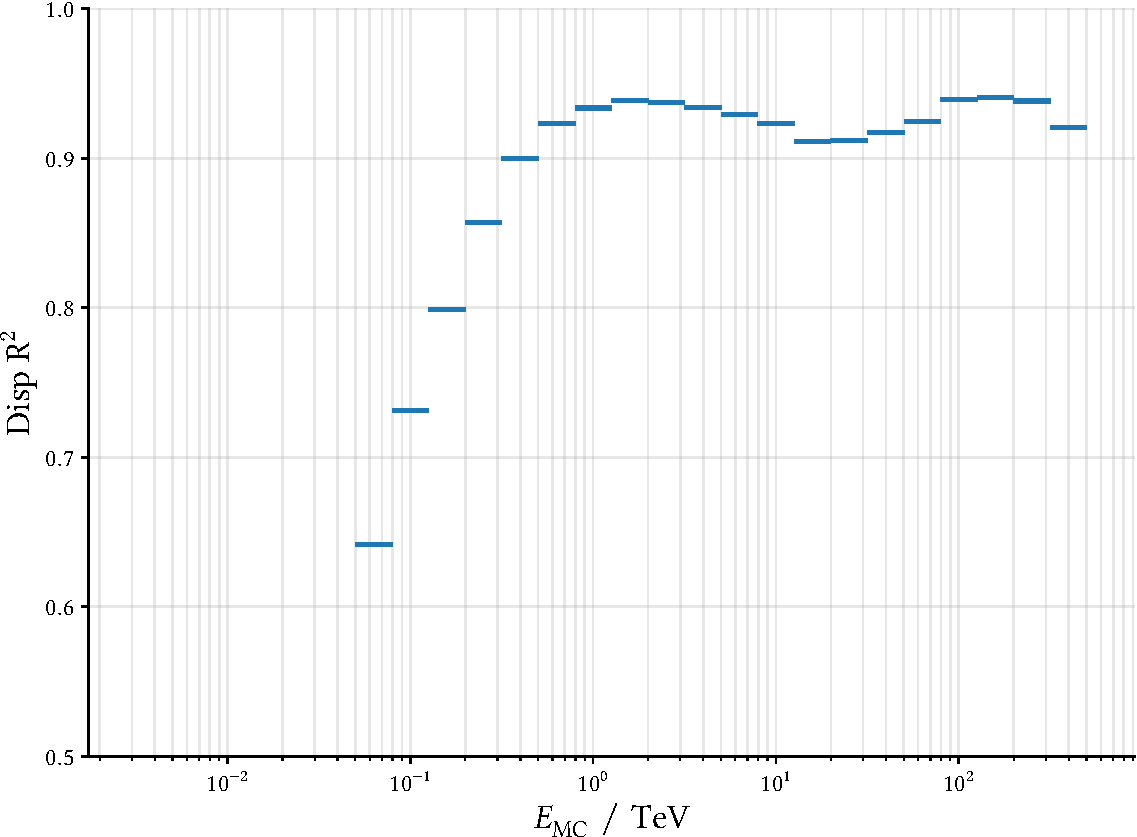
\includegraphics[width=\linewidth]{../analysis/plots/disp_test_r2_equal_sized.pdf} 
        \caption{R2-Score for the DISP-estimation}
    \end{subfigure}
    \begin{subfigure}{0.45\textwidth}
        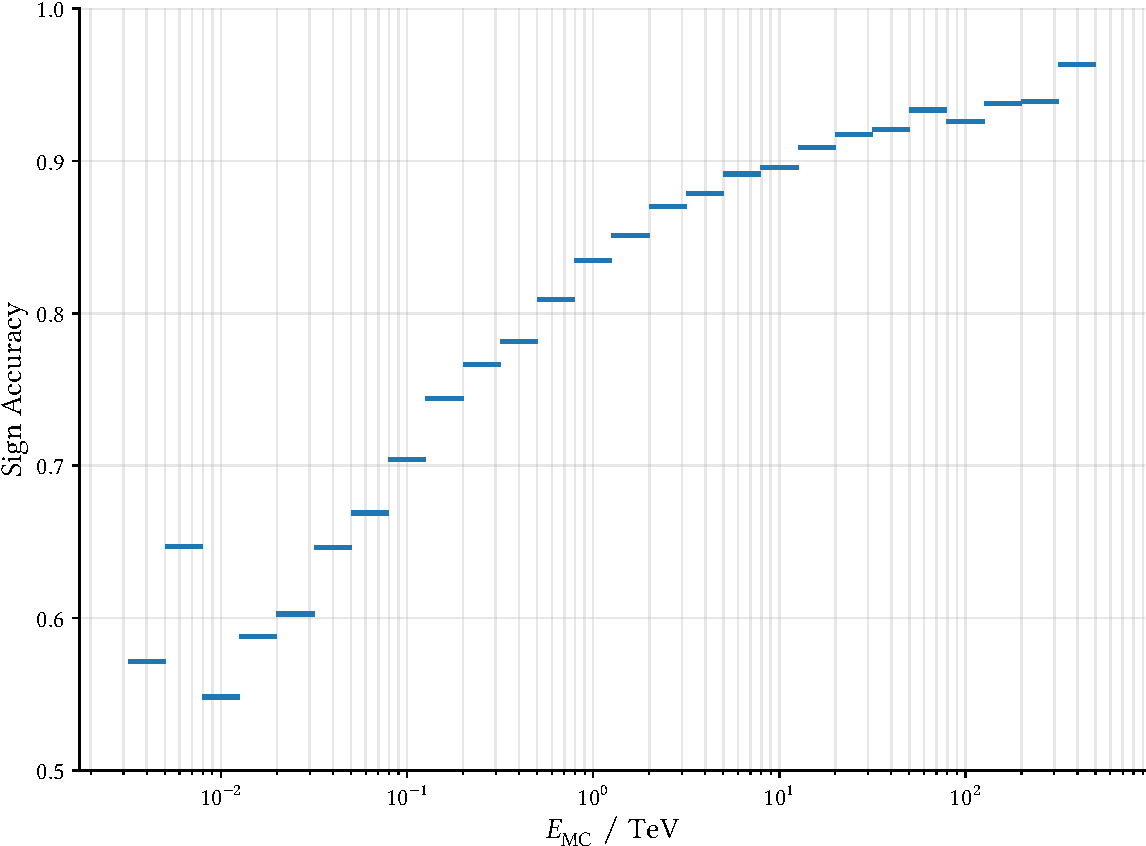
\includegraphics[width=\linewidth]{../analysis/plots/disp_test_acc_equal_sized.pdf}
        \caption{Accuracy for the SIGN-estimation}
    \end{subfigure}
    \caption{
    	Performance of the DISP- and SIGN-estimation algorithm on the diffuse test-dataset.
	Both model predictions improve with higher energies and saturate
	at $\approx\num{0.95}$ for the $R2$ and accuracy respectively.
    The DISP-performance shows a dip in the energy range of \SI{3}{\tera\electronvolt}
    up to \SI{70}{\tera\electronvolt}, that cannot be explained at this point.}
    \label{fig:disp_test_perf}
\end{figure}

\begin{figure}
    \centering
    \captionsetup{width=0.9\linewidth}
    \begin{subfigure}{0.45\textwidth}
        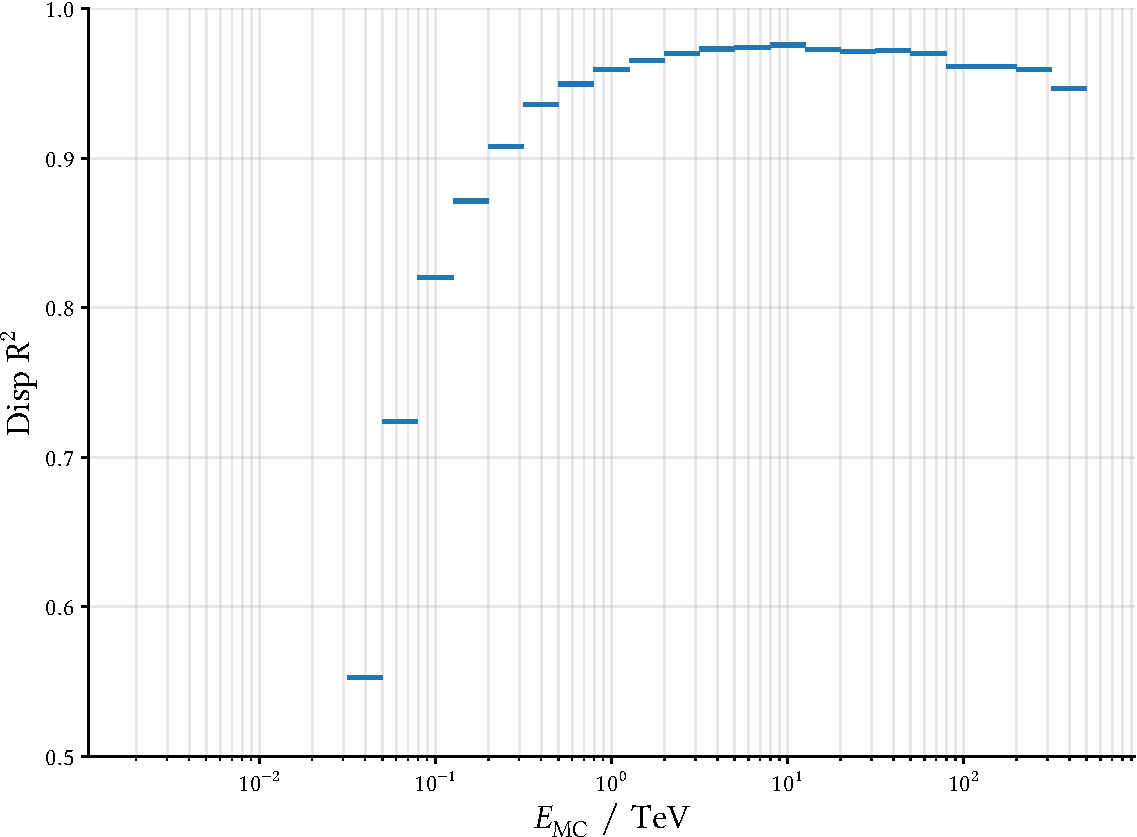
\includegraphics[width=\linewidth]{../analysis/plots/disp_gamma_r2_equal_sized.pdf} 
        \caption{R2-Score for the DISP-estimation}
    \end{subfigure}
    \begin{subfigure}{0.45\textwidth}
        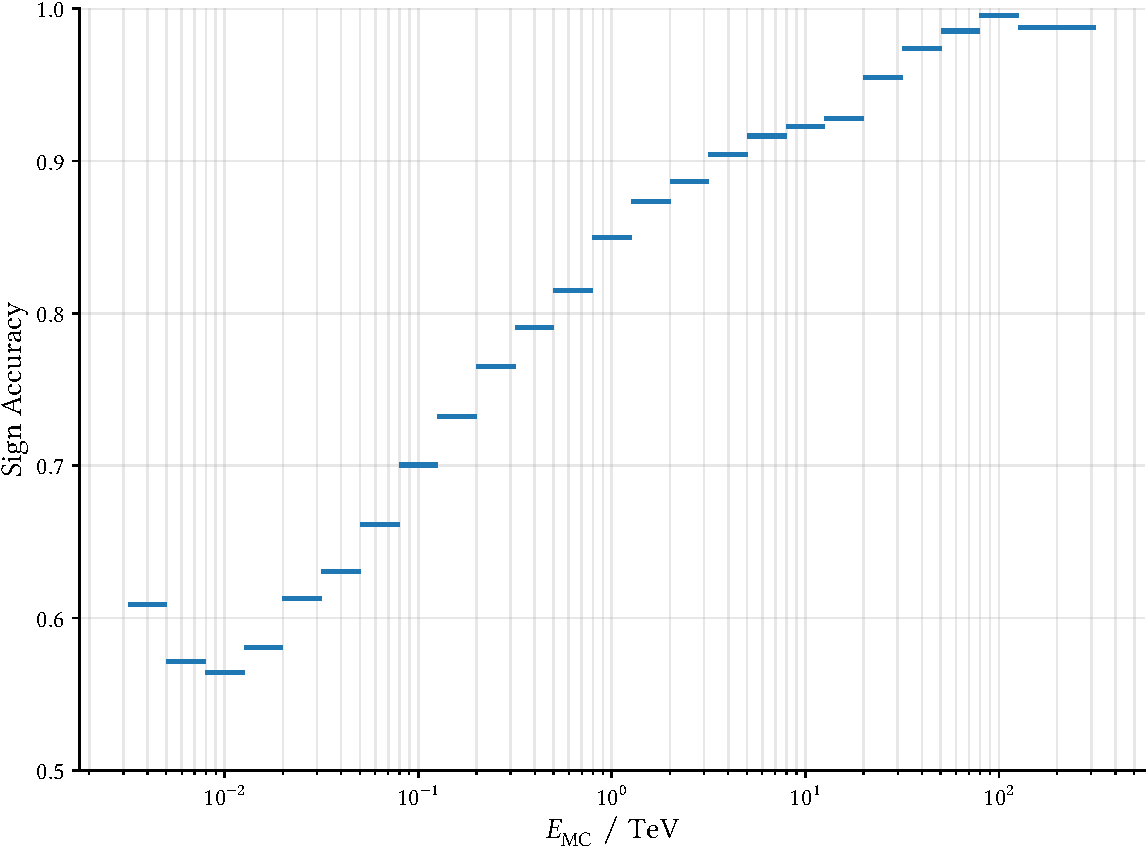
\includegraphics[width=\linewidth]{../analysis/plots/disp_gamma_acc_equal_sized.pdf}
        \caption{SIGN-accuracy}
    \end{subfigure}
    \caption{
	Performance of the DISP- and SIGN-estimation algorithm on the pointlike dataset.
    The R2-score of the DISP predictions shows a different form on pointlike
	compared to diffuse gammas: The performance generally seems to be a bit better, 
	with saturation closer to 1. The dip in the DISP-performance is gone, but the highest energy bins
	show a decreasing performance.
    The accuracy of the SIGN-predictions looks generally similar to the one on diffuse data,
    but with better performance in most bins.}
    \label{fig:disp_gamma_perf}
\end{figure}

The error of the resulting (monoscopic) source position reconstruction 
can be seen in figures \ref{fig:sens_telescope_test} and \ref{fig:sens_telescope}
respectively.
One can derive - in accordance to the previously discussed metrics - 
that both the DISP and SIGN predictions improves with increasing energies.
The predictions get worse at around the energies, where the $R2$-score
on the DISP-predictions saturates and decays.

\begin{figure}
    \centering
    \captionsetup{width=0.9\linewidth}
    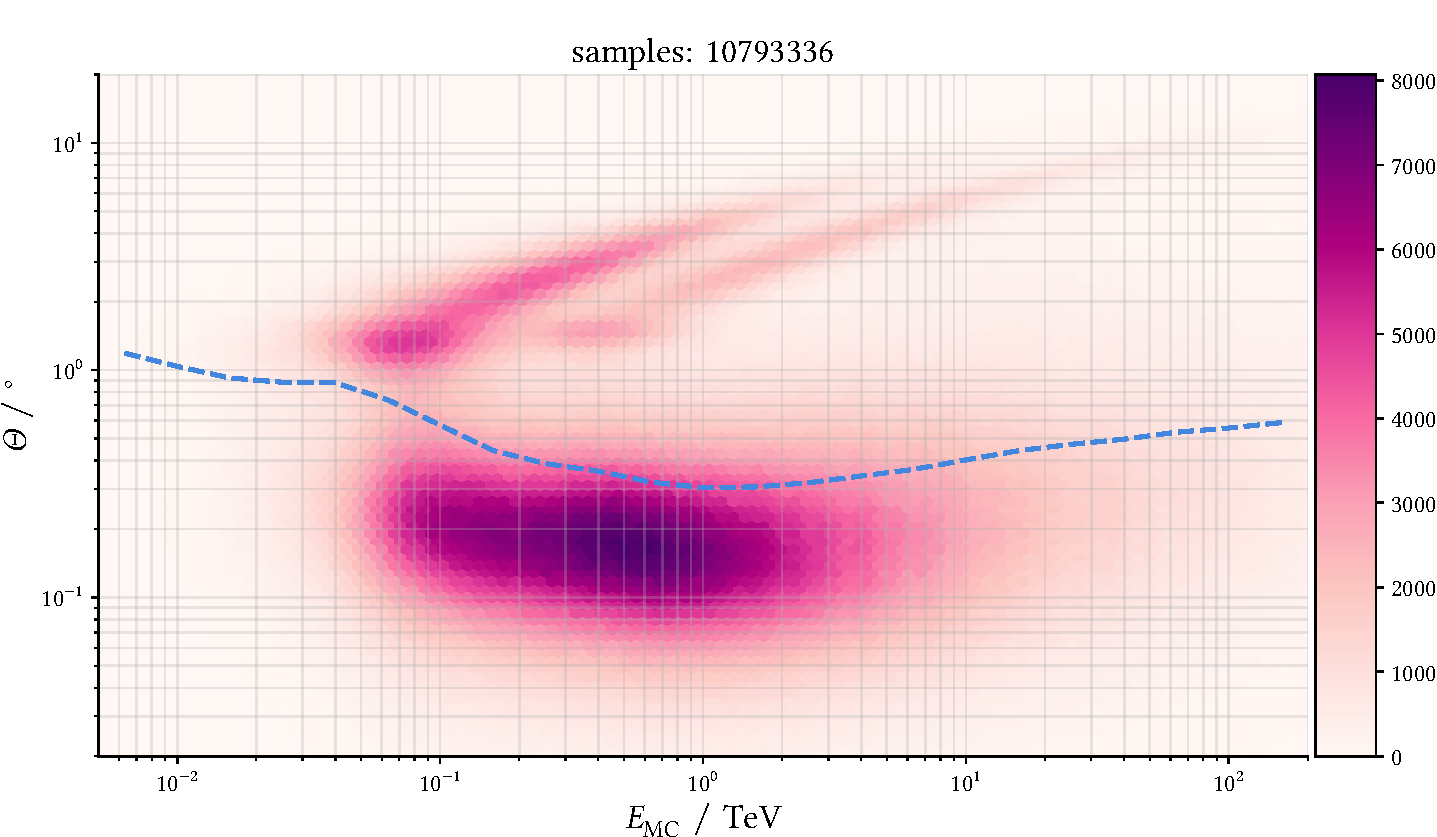
\includegraphics[width=.9\textwidth]{../analysis/plots/test/tel_vs_energy.pdf}
    \caption{Per telescope predictions for the source position on the diffuse test set.
    The blue-dotted line shows the 68\% containment. 
    A lot of misclassified events at the lower energies
    lead to a second population above the main one.
    The misclassification rate decreases with higher energies 
    in accordance to figure \ref{fig:disp_test_perf}.
    For very high energies the predictions do not improve despite the lower 
    misclassification rate, fitting our earlier conclusions regarding the DISP-performance.}
    \label{fig:sens_telescope_test}
\end{figure}

\begin{figure}
    \centering
    \captionsetup{width=0.9\linewidth}
    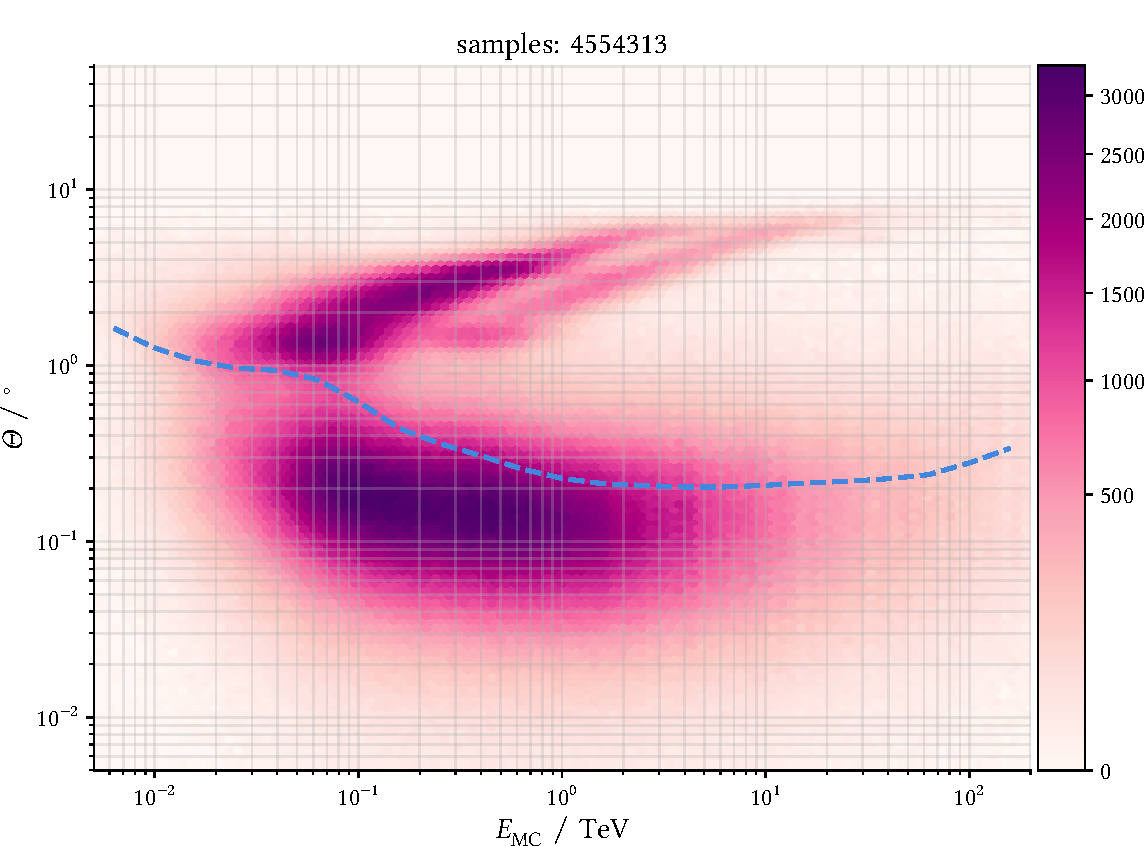
\includegraphics[width=.9\textwidth]{../analysis/plots/gamma/tel_vs_energy.pdf}
    \caption{Per telescope predictions for the source position on the pointlike 
    gamma dataset. The blue-dotted line shows the 68\% containment. 
    Similar conclusions as from figure \ref{fig:sens_telescope_test} can be drawn
    with respect to the DISP and SIGN performance.}
    \label{fig:sens_telescope}
\end{figure}


The feature importances for the DISP model can be seen in figure \ref{fig:disp_features},
the one for the SIGN model in figure \ref{fig:sign_features}.
For the DISP-model the reconstructed interaction heigth and core position
show the most impact alongside the features, that describe light content and size of
the shower ellipse. 
The SIGN-predictions on the other hand are dominated by the observed 
$skewness$ and $slope$.

\begin{figure}
	\centering
    \captionsetup{width=0.9\linewidth}
	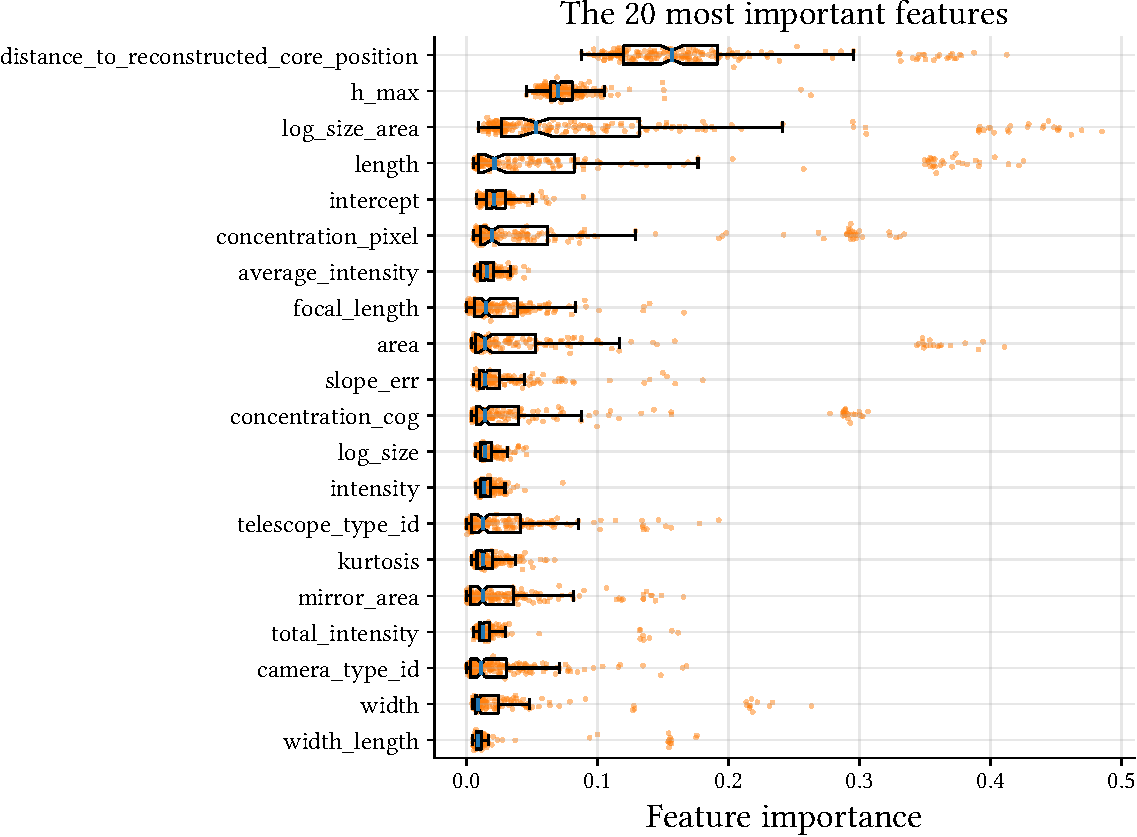
\includegraphics[width=0.9\textwidth]{../analysis/plots/disp_features.pdf}
	\caption{
	    Feature importance of the random forest for the DISP model.
	    The added stereoscopic features have high influence on the prediction.
    	From the monoscopic features the specifically constructed feature
    	$log\_size\_area$ seems to include the most information on average.
        Looking at the distribution of the individual feature importances, it 
        can be derived that the range of important featrues is bigger than this list
        with especially the $concentration$-features, the $area$, $width$ and $length$
        being of high importance to the model as well.}
	\label{fig:disp_features}
\end{figure}

\begin{figure}
	\centering
    \captionsetup{width=0.9\linewidth}
	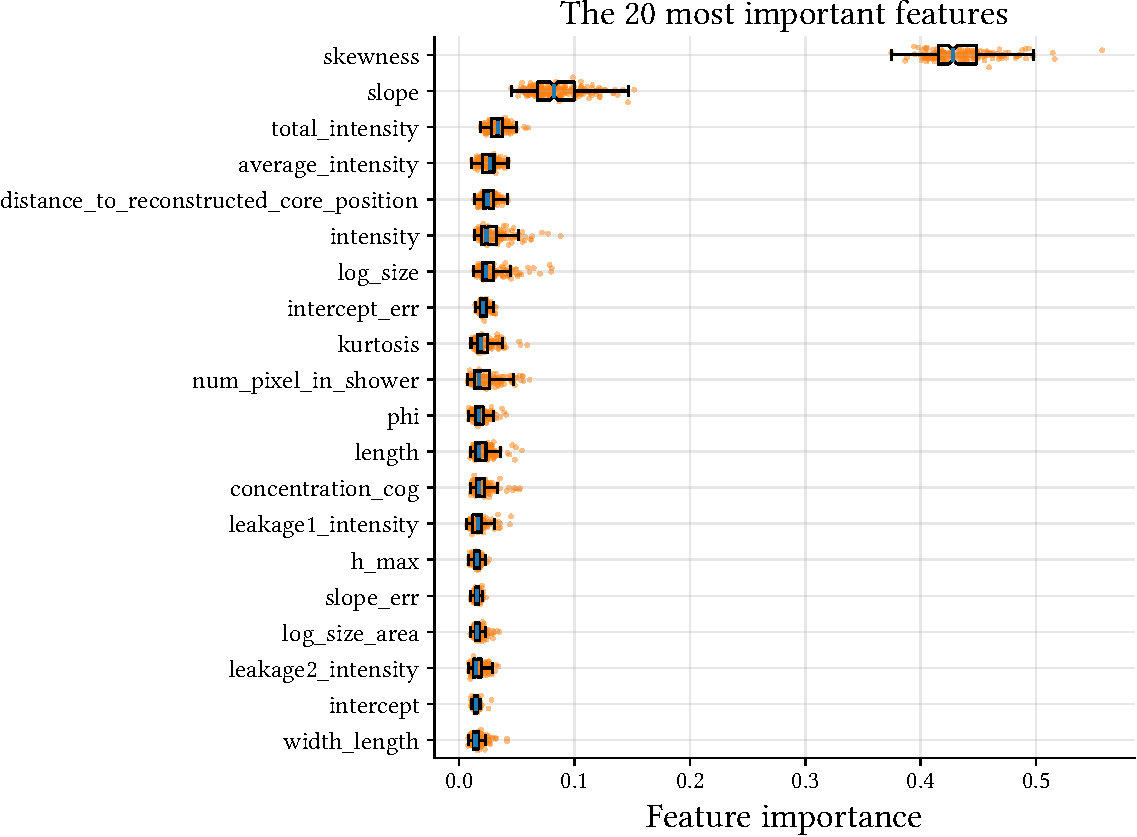
\includegraphics[width=0.9\textwidth]{../analysis/plots/sign_features.pdf}
	\caption{Feature importance of the random forest for the SIGN model.
	        The most influential features to the prediction are by far the higher-order moments $skewness$
            and $slope$. The stereoscopic features do not provide much information,
            which is expected as the head-/tail-ambiguation is entirely an artefact produced
            in the camera frame. Other features provide very little information, with all
            the features describing the light content being highly ranked amongst those.
            The hillas parameters seem to be of little relevance for the SIGN prediction.}
	\label{fig:sign_features}
\end{figure}




\subsection{Stereoscopic Predictions}

The results of the baseline median DISP+SIGN-prediction
compared to the existing HillasReconstructor can be seen in figure \ref{fig:stereo_median_energy}
and \ref{fig:stereo_median_multi}.

At each energy the HillasReconstructor performs considerably better.
One can derive that the median predictions do not improve considerably after
\SI{3}{\tera\electronvolt} and get worse after \SI{10}{\tera\electronvolt}.
The HillasReconstructor shows a similar stauration at the highest energies,
but without the prominently decaying performance of the median peridctions.
Due to the low statistics we can not get to statistically relevant
conclusions in this region however.

The HillasReconstructor also shows a pronounced bump in the range of \SI{200}{\giga\electronvolt}
to \SI{1}{\tera\electronvolt}. 
This has been observed earlier and seems to correlate with 
a lot of low multiplicity events in the crossover region from LSTs to MSTs \cite{kai? max?}.

Looking at the performance over multiplicity we can conclude that the median predictions
do not scale as well with higher multiplicities, so that the performance gap increases with
the multiplicities going up.

\begin{figure}
    \centering
    \captionsetup{width=0.9\linewidth}
    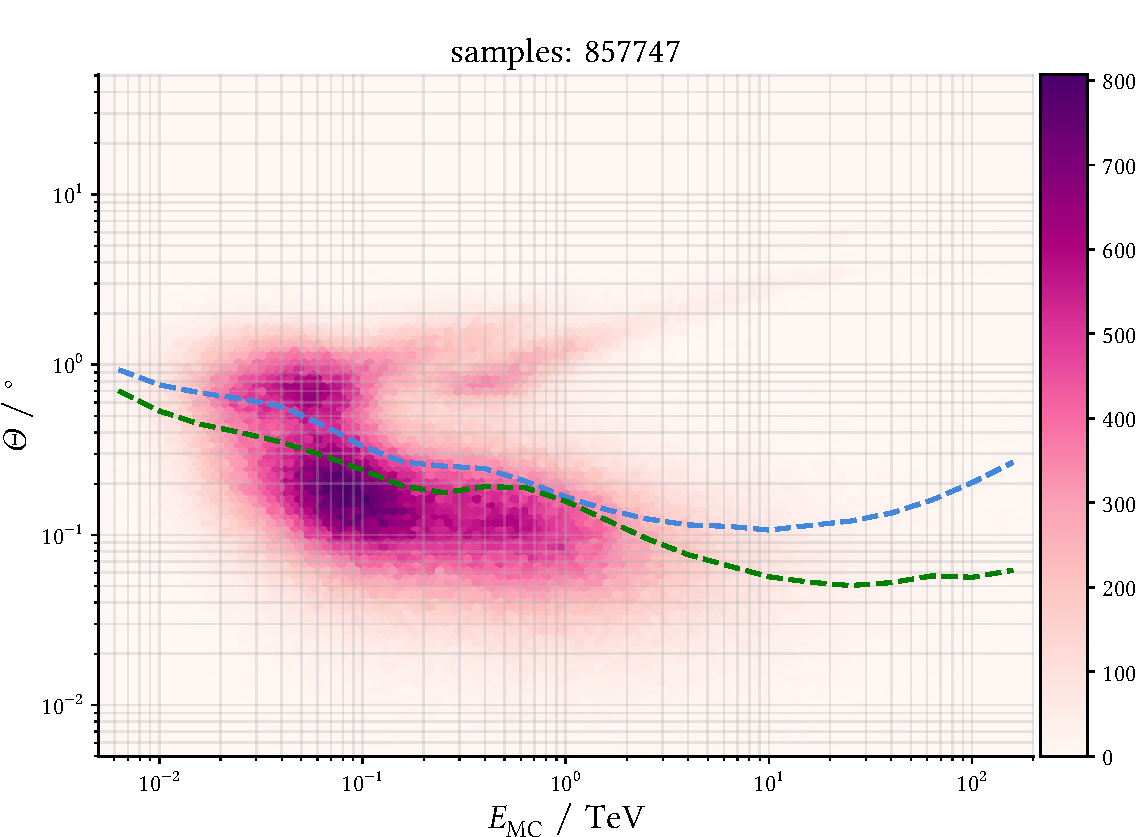
\includegraphics[width=0.9\linewidth]{../analysis/plots/gamma/median_vs_energy.pdf} 
    \caption{Distance between predicted and true position over true energy as obtained by taking the median of
    the DISP+SIGN predictions.
    The binned results refer to the median DISP+SIGN-predictions. The blue line shows the 
    68\% containment of these results. The green line refers to the 68\%
    results of the HillasReconstructor which are not shown in bins.
    Despite the short bump in the range of \SI{200}{\giga\electronvolt}
    to \SI{1}{\tera\electronvolt} the HillasReconstructor outperforms the median predictions
    massively.}
    \label{fig:stereo_median_energy}
\end{figure}

\begin{figure}
    \centering
    \captionsetup{width=0.9\linewidth}
    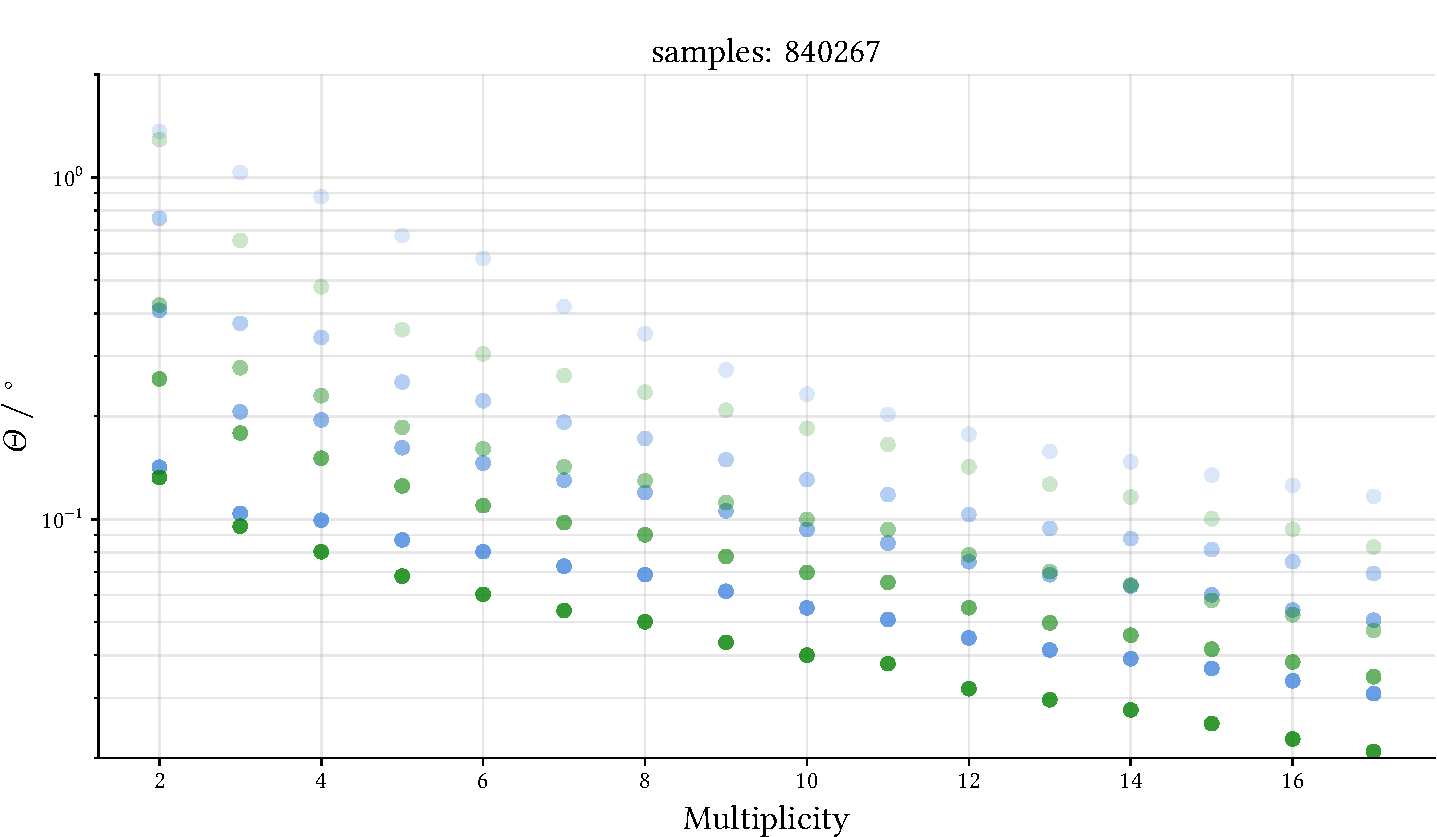
\includegraphics[width=0.9\linewidth]{../analysis/plots/gamma/median_vs_multi_comp.pdf}
    \caption{Distance between predicted and true position over event multiplicity. Both algorithms require
    multiplicities $\geq 2$. Higher multiplicity events are cut off, because 
    statistical fluctuations dominate as not many events are recorded.
    Blue and green refer to the median predictions (blue) and the HillasReconstructor (green) predictions.
    The different lines refer to the 25,50,68 and 90\% percentiles with 
    lowering alpha.
    The median predictions are worse at every multiplicity and the gap increases with higher event multiplicity.}
    \label{fig:stereo_median_multi}
\end{figure}

The results of the more sophisticated iterative DISP-approach can be seen in figures
\ref{fig:stereo_magic_energy} and \ref{fig:stereo_magic_multi}.
Compared to the median predictions, the completely misreconstructed events are almost
completely resolved and the 68\% percentile is much improved throughout the complete energy range besides 
the very highest energies. At this point the error of the DISP-prediction is probably limiting and the 
Hillas-reconstructor leads to much better results.
At the lower energy range our approach seems to be working pretty well, 
slightly outperforming the HillasReconstructor.

When looking at the multiplicity-plot, we see a similar picture as before but with 
better results. At high event multiplicities the Hillas-reconstructor 
leads to better results. Improvements can be seen especially at 2- and 3-multiplicity 
events. In the case of 2 telescopes the iterative approach reduces to the 
base Magic algorithm without the cut for too distant predictions.
The HillasReconstructor on the other hand does not work too well with 2 
triggered telescopes, with 3 triggered telescopes leading to much better results 
already especially at the 90\% percentile.


\begin{figure}
    \centering
    \captionsetup{width=0.9\linewidth}
    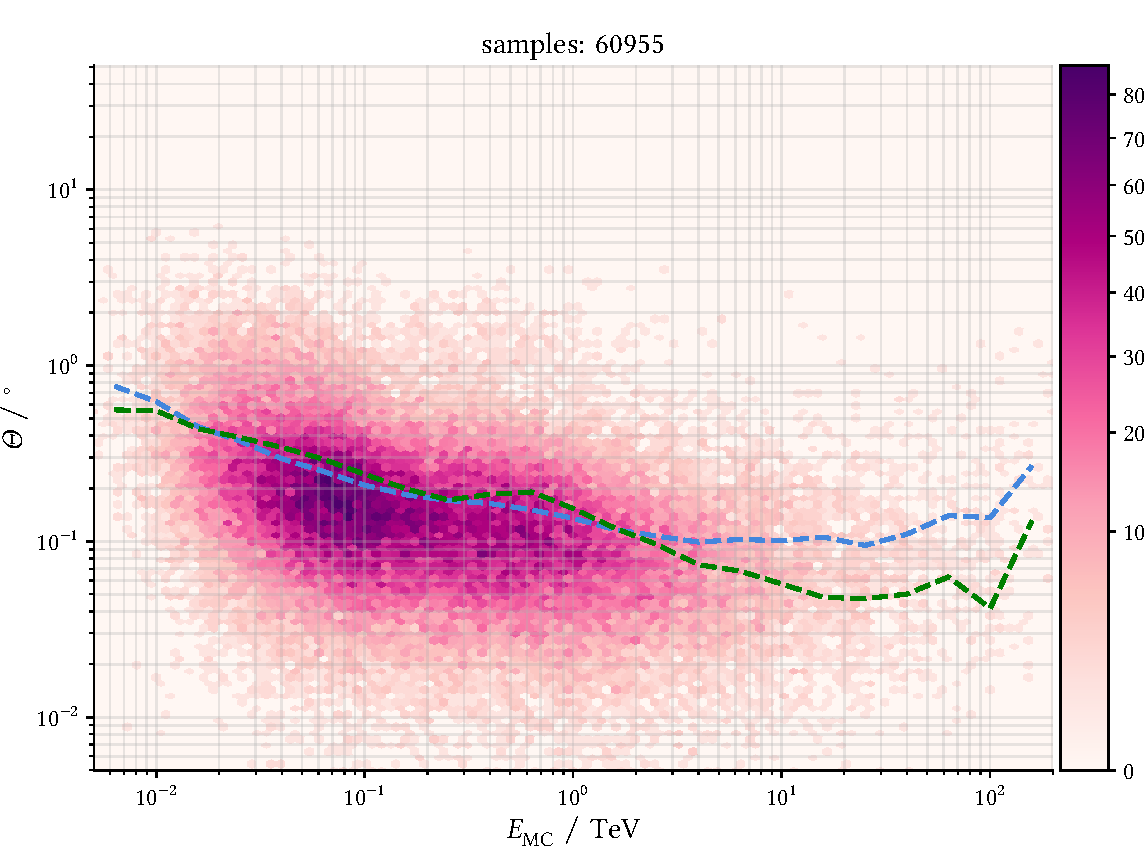
\includegraphics[width=0.9\linewidth]{../analysis/plots/gamma/pairwise_median_100_vs_energy.pdf} 
    \caption{Distance between predicted and true position over true event energy as obtained with our
    iterative DISP approach.
    The binned results refer to the iterative DISP-predictions. The blue line shows the 
    68\% containment of these results. The green line refers to the 68\%
    results of the HillasReconstructor which are not shown in bins.
    The DISP-approach outperforms the HillasReconstructor up to
    $\approx \SI{2}{\tera\electronvolt}$.
    At higher energies we see the same behaviour as earlier, with the performance actually
    decreasing again.}
    \label{fig:stereo_magic_energy}
\end{figure}

\begin{figure}
    \centering
    \captionsetup{width=0.9\linewidth}
    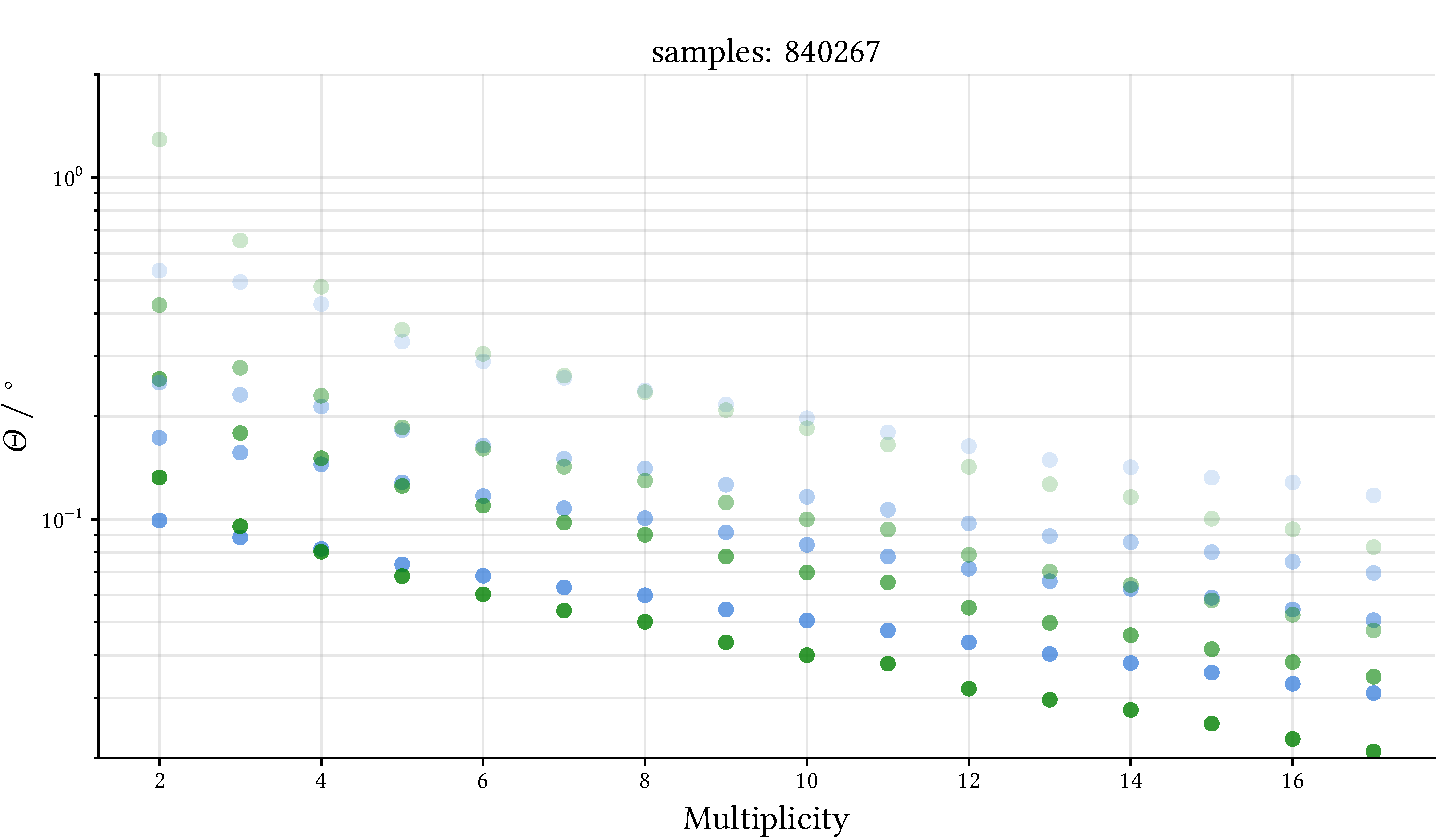
\includegraphics[width=0.9\linewidth]{../analysis/plots/gamma/pairwise_median_100_vs_multi_comp.pdf}
    \caption{Distance between predicted and true position over event multiplicity. Both algorithms require
    multiplicities $\geq 2$. Higher multiplicity events are cut off, because 
    statistical fluctuations dominate as not many events are recorded.
    Blue and green refer to the median predictions and the HillasReconstructor predictions.
    The different lines refer to the 25,50,68 and 90\% percentiles with 
    lowering alpha.
    For low multiplicities the combined DISP-predictions are superiour, 
    for high multiplicities the HillasReconstructor results win out.
    The breakeven point seems to be at 4-6 telescopes, depending on 
    which percentiles have more weight to the analysis.}
    \label{fig:stereo_magic_multi}
\end{figure}


\section{Stereoscopic Predictions with Hadroness Cut}

Based on the performance of the gamma-/hadron-separation model 
(see again \ref{fig:gh_fscore})
we set the gammaness cut to be at a mean score of \num{0.82}.
This means that all events, where the average of the telescope predictions
is less than \num{0.82}, get discarded.

With this cut \num{272441} of the \num{955317} events remain on array-event level, 
which equals an efficiency of \num{28.52}\%.

We apply the DISP-model with our iterative approach
the same way as in the earlier steps and compare the results to the HillasReconstructor
again, of which the resulty can be ssen in figures \ref{fig:stereo_magic_energy_cut}
and \ref{fig:stereo_magic_multi_cut}.

\begin{figure}
    \centering
    \captionsetup{width=0.9\linewidth}
    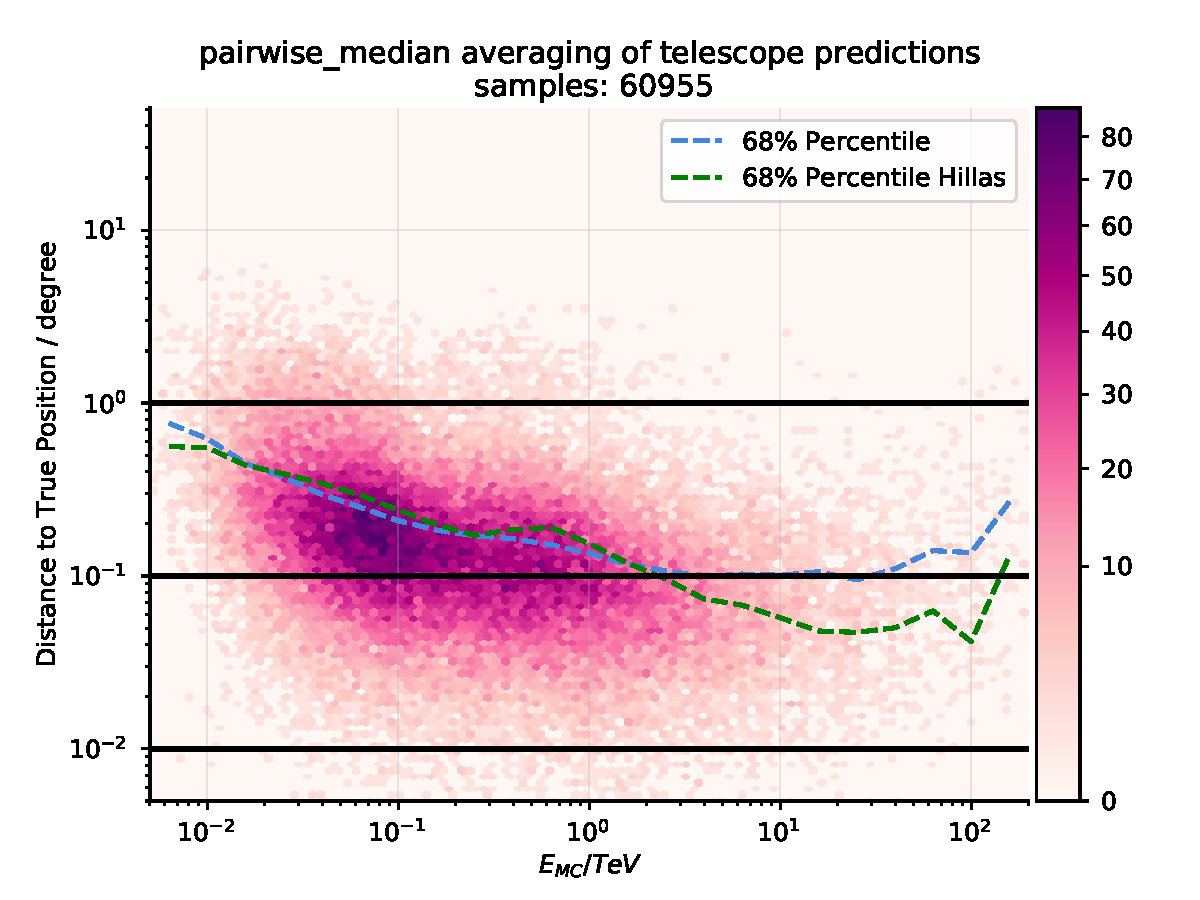
\includegraphics[width=0.9\linewidth]{../analysis/plots/gamma_cut/pairwise_median_100_vs_energy.pdf} 
    \caption{Distance between predicted and true position over true event energy as obtained with our
    iterative DISP approach after applying the hadroness cut.
    The cut seems to remove mainly low energy events. The predictions for both
    algorithms are much improved over the complete energy range compared to figure \ref{fig:stereo_magic_energy}.
    As before the DISP-approach works better for low wnergies and diverges for very high energies.}
    \label{fig:stereo_magic_energy_cut}
\end{figure}

\begin{figure}
    \centering
    \captionsetup{width=0.9\linewidth}
    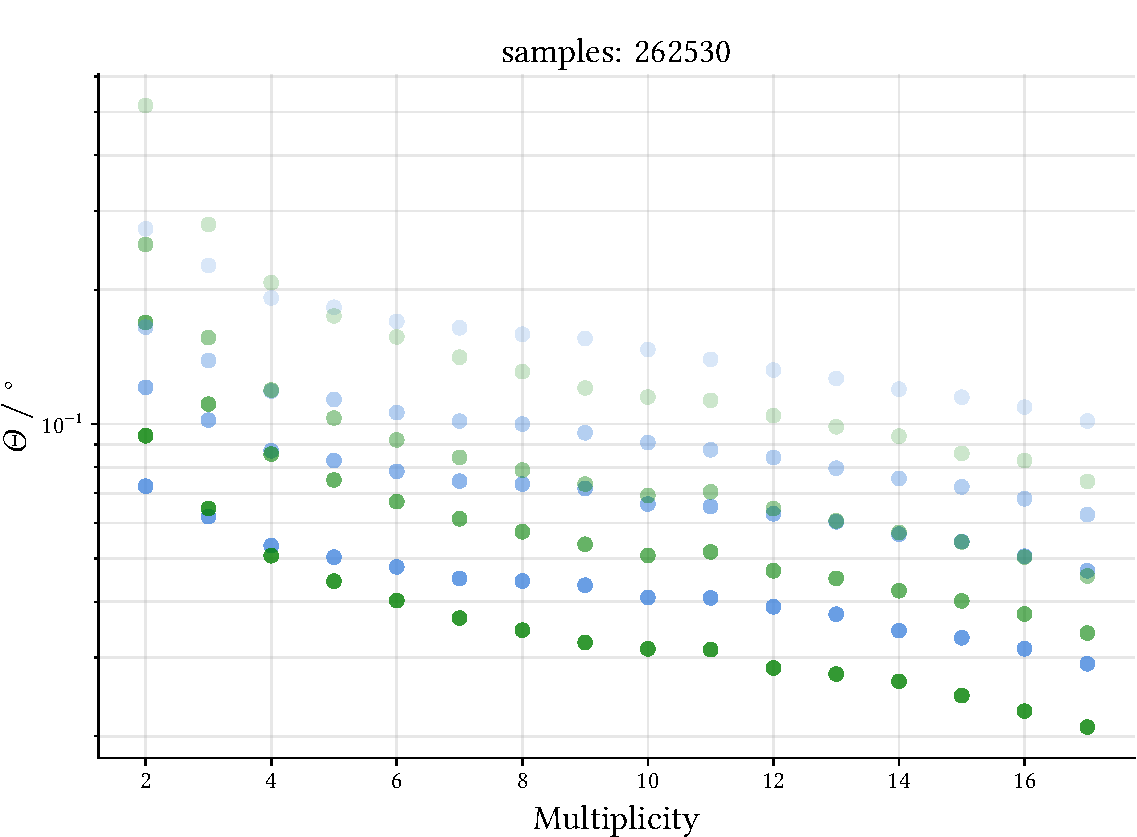
\includegraphics[width=0.9\linewidth]{../analysis/plots/gamma_cut/pairwise_median_100_vs_multi_comp.pdf}
    \caption{Distance between predicted and true position over event multiplicity after applying the hadroness cut. Both algorithms require
    multiplicities $\geq 2$. Compared to the results in figure \ref{fig:stereo_multi_energy}, 
    the HillasReconstructor seems to have gained more performance at the low multiplicities, now strictly outperforming the 
    DISP-approach on multiplicities of 5 and higher.}
    \label{fig:stereo_magic_multi_cut}
\end{figure}

\iffalse
\section{LST only}
To simulate early operation stages where the LST1 is the only fully functional 
telescope, the analysis is limited to only the single LST with 
the telescope\_id 4.

This means that we do not have a baseline Hillas Reconstructor as we can not use
stereoscopy and each array event holds exactly one telescope event.
We expect to
get a similar sensitivity as in the earlier figure \ref{fig:sens_telescope}.

We also try to limit the training data on this particular telescope.
This will leave us with far less training samples, but hopefully
a better model?????

HOW DOES THE PERFORMANCE CHANGE?
THIS REQUIRES MORE EVENTS AND MAYBE MORE LSTS FOR TRAINING?
COMPARE TO APPLYING THE NORMAL MODEL

\begin{figure}
    \begin{subfigure}{0.45\textwidth}
        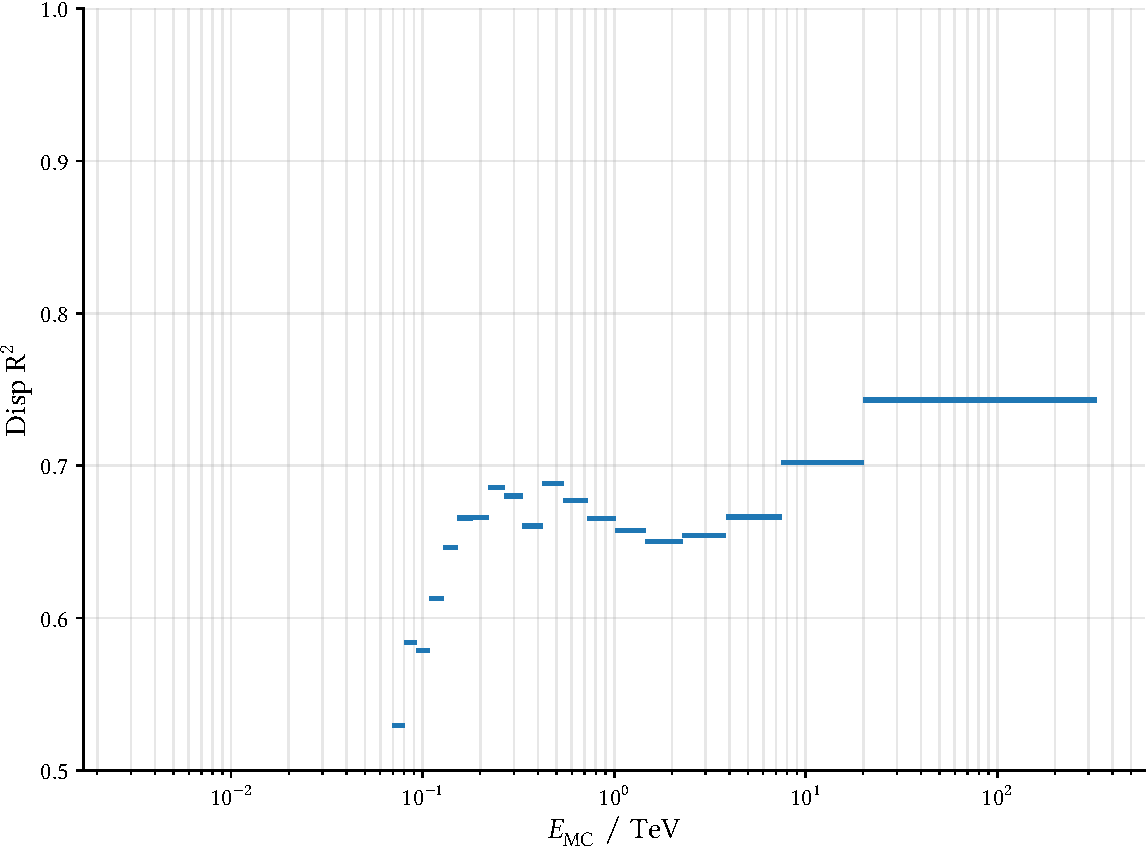
\includegraphics[width=0.9\linewidth]{../analysis/plots/disp_test_mono_lst_r2_equal_filled.pdf} 
        \caption{R2-Score for the DISP-estimation}
    \end{subfigure}
    \begin{subfigure}{0.45\textwidth}
        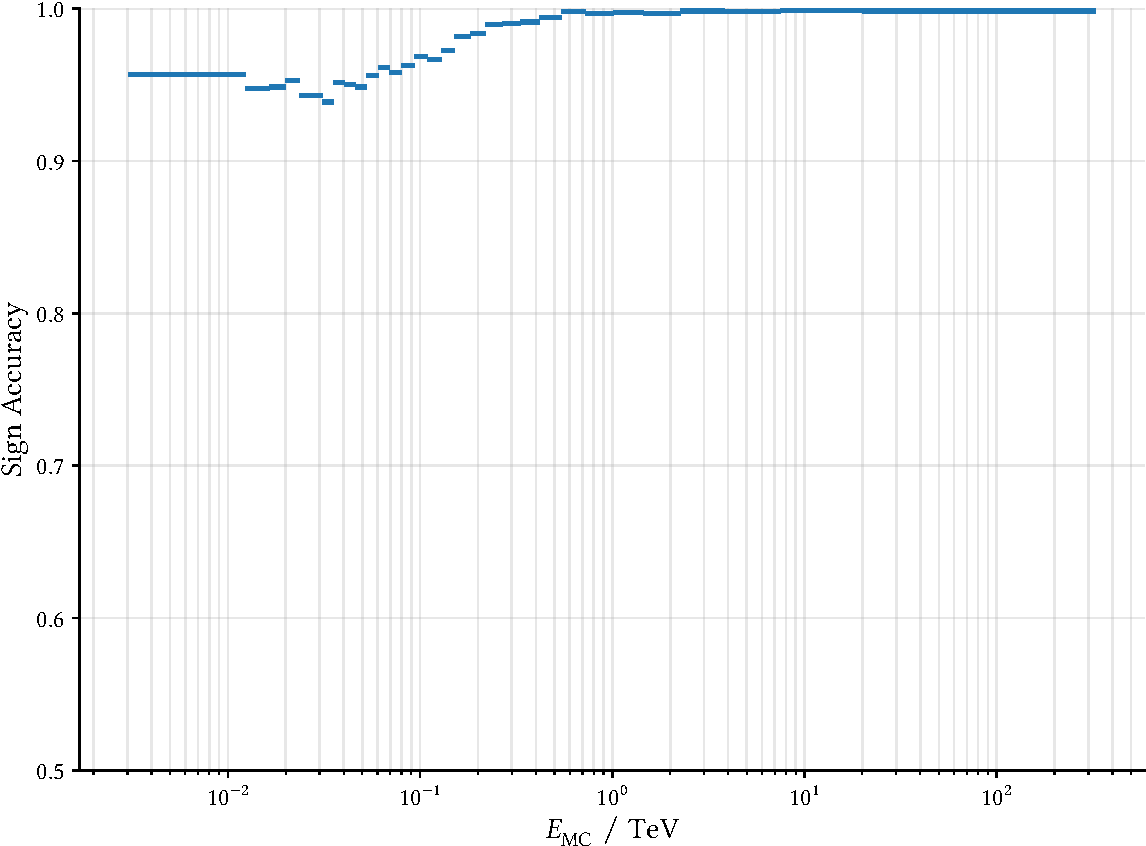
\includegraphics[width=0.9\linewidth]{../analysis/plots/disp_test_mono_lst_acc_equal_filled.pdf}
        \caption{SIGN-accuracy}
    \end{subfigure}
    \caption{Performance of the DISP- and SIGN-estimation algorithm on the test-dataset.}
    \label{fig:disp_test_perf}
\end{figure}

\begin{figure}
    \begin{subfigure}{0.45\textwidth}
        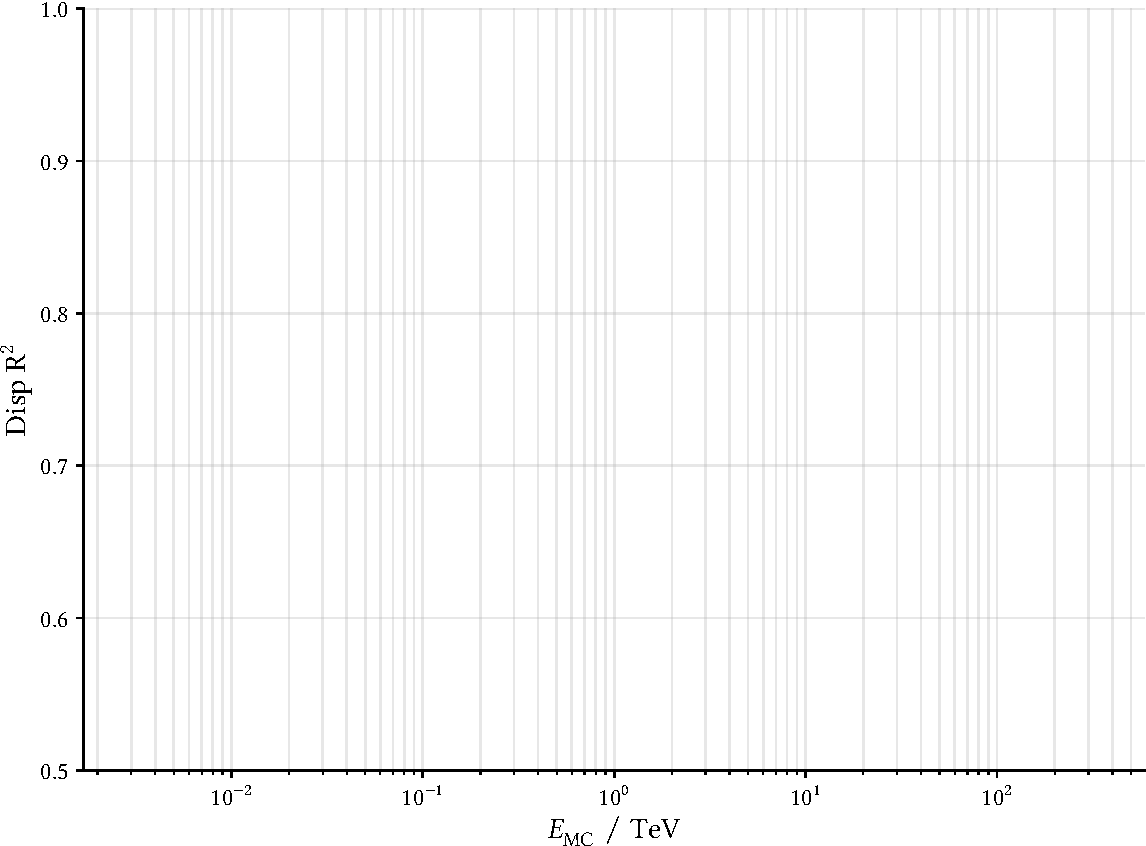
\includegraphics[width=0.9\linewidth]{../analysis/plots/disp_gamma_mono_lst_r2_equal_filled.pdf} 
        \caption{R2-Score for the DISP-estimation}
    \end{subfigure}
    \begin{subfigure}{0.45\textwidth}
        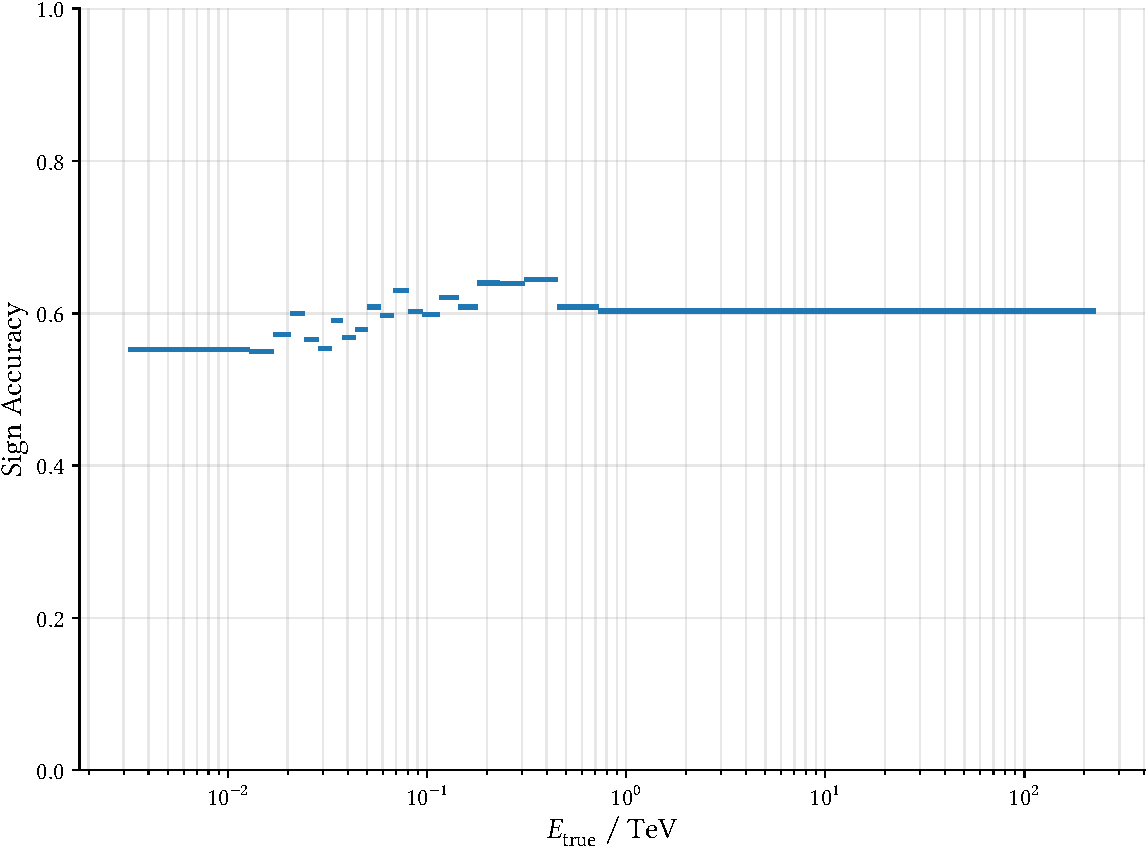
\includegraphics[width=0.9\linewidth]{../analysis/plots/disp_gamma_mono_lst_acc_equal_filled.pdf}
        \caption{SIGN-accuracy}
    \end{subfigure}
    \caption{Performance of the DISP- and SIGN-estimation algorithm on the pointlike dataset..}
    \label{fig:disp_gamma_perf}
\end{figure}

Looks decent, energy obviously limited bc LST.

\fi